\chapter{Electronic Excited States}

\begin{quote}
  "The XXIst century might be very well the century of light. Understanding and controlling photoexcited systems will be crucial for future research in many branches of optics and photonics."
  \begin{flushright}
    \small{--- \textit{L. González, D. Escudero, L. Serrano-Andrés (2011) \cite{Gon2012} }}
  \end{flushright}
\end{quote}

A quantum system is said to be in an \emph{excited state} if that state is at a higher energy level than the ground state, for example by absorption of one or more light quanta. While computing ground state properties has become routine even for larger molecules, the extension of the standard models to excited state properties is an active field of research. Triggered by the development of complex, high-resolution spectroscopic techniques such as X-ray spectroscopy \cite{Nor2018a}, and advances in photochemistry \cite{Gon2012}, the demand for accurate and computational methods of excited states has been steadily increasing. Electronic spectra are often very difficult to interpret, and \emph{computational spectroscopy} has emerged as an important tool to explain the underlying mechanisms.

Excited states are notoriously difficult to model, and similarly to their ground state analogs, there is no single method to rule them all. Over the years, many different approaches have been proposed, each with their strengths and weaknesses. This section will go over the most popular, single-reference methods  available, with a focus on the algebraic diagrammatic construction method. 

\section{Nature of Excited States}

The potential energy landscape of electronic excited states is complex and governed by various absorption and decay mechanisms. Excitations are generally grouped into three categories:
\begin{enumerate}
\item \emph{Valence excitations}, where valence electrons are excited into (local) higher lying unoccupied orbitals above the Fermi level
\item \emph{Rydberg excitations}, where electrons are excited into very diffuse orbitals around the molecule
\item \emph{Charge transfer excitations} (CT), where electrons are excited to different parts of the molecule or different molecules entirely. 
\end{enumerate}

Excited states typically have lifetimes and decay back to the ground state via several different mechanisms. Figure \ref{fig:PESEX} illustrates the different processes. The notation $S$, $D$, $T$ ... is used to denote singlet, doublet, triplet ... states and the subscripts indicate the energy level, where 0 is the ground state, 1 is the first excited state for the given spin symmetry, 2 is the second excited state etc. The transition from the ground state $S_0$ to the excited state $S_1$ on the same reaction coordinate is known as a \emph{vertical excitation}. The excited state may be in a higher vibrational state at that reaction coordinate (indicated by the lines within the potential wells), and relax to the lowest level. The difference between these two points is known as the \emph{reorganization energy}, and the difference between the lowest vibrational states of $S_0$ and the excited state is known as the \emph{adiabatic excitation} energy. The 
molecule returns to the ground state by emitting a photon in a process known as \emph{fluorescence}. 

Surfaces of different states may cross at specific reaction coordinates. The crossing between states with different multiplicity (e.g. S$_1$ to T$_1$) is known as an inter-system crossing (ISC). The process between two states where the crossing takes place between molecules of the same spin-symmetry is known as \emph{internal conversion} (IC), and takes place at a \emph{conical intersection} (CoIn). The S$_1$ excited state can cross over to the T$_1$ state via an ISC which then decays in a process known as \emph{phosphorescence}, or it can decay radiation-less via the CoIn. At the ISC and CoIn, the Born-Oppenheimer approximation breaks down due to non-adiabatic coupling between electrons and nuclei. ISCs and CoIns are central to describing the dynamics in photochemical events \cite{Mig2008,Mat2011,Kim2015,Zhu2016}.

For the sake of brevity, this chapter will focus on the computational of vertical excitation energies only.

\begin{figure}
\centering
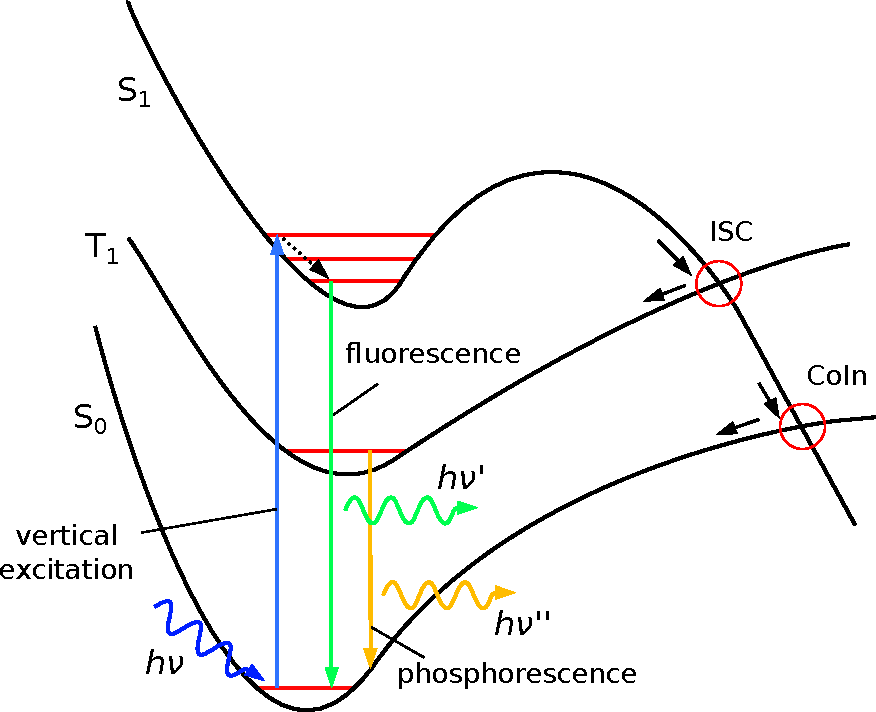
\includegraphics[scale=0.8]{Pics/PESEX}
\caption{Potential energy surface of a chemical system depicting the major pathways encountered in spectroscopy and photochemistry.}
\label{fig:PESEX}
\end{figure}

\section{Explicit Optimization of the Excited State Wave Function}

One of the conceptually simplest approaches for obtaining information on excited states is explicit optimization of the excited wave function. The excitation energy is then directly computed by taking the difference between the ground state energy and the energy of excited state $i$
\begin{equation}
E_{0\rightarrow i} = E_i - E_0 
\end{equation} 
\noindent Any ground state model discussed in the previous chapter can be used. This approach to excited states is known by different names, depending on which approximation is used. Generally, the Greek letter $\Delta$ is just prepended to the method name, giving $\Delta$SCF or $\Delta$HF for Hartree-Fock \cite{Bag1965,Deu1976,Amb2019}, $\Delta$KS (Kohn-Sham) or $\Delta$DFT for DFT \cite{Tri1999,Tak2003,Bes2009}, and so on. At the moment of writing, excitation energies are also routinely computed using $\Delta$MP$n$ \cite{Hol2011}, $\Delta$CI, $\Delta$MCSCF \cite{Sch2015} and $\Delta$CC \cite{Hol2011,Zhe2019}. From here on out, $\Delta$X will be used as an umbrella term to group all aforementioned terms. 

Despite the simplicity of the $\Delta$X methods, obtaining a solution to the KS or HF equations for higher energy states is non-trivial. By the variational principle, the SCF method finds the lowest energy solution. A HF type excited wave function may therefore collapse to that lowest energy solution during the SCF procedure (variational collapse). For small symmetric molecules, it is possible to converge excited states if they have a different spin multiplicity or spatial point group to the ground state. If the ground and excited state have the same symmetry however, this approach will not work. This technical difficulty was one of reasons why $\Delta$X methods never gained much ground compared to more sophisticated methods.

In 2008, Gilbert et al. \cite{Gil2008} proposed a modification the SCF procedure that prevents variational collapse, known as the \emph{maximum overlap method} (MOM). On each iteration, the new guess orbitals are obtained by diagonalization of the Fock matrix which is constructed using the old coefficients
\begin{equation}
\mbf{F}(\mbf{C}^{old})\mbf{C}^{new} = \mbf{S}\mbf{C}^{new}\epsilon
\end{equation}
\noindent At this step, it is possible to decide which of those new orbitals are actually occupied. Normally, the $n_{occ}$ eigenvectors with the lowest eigenvalues are chosen as the new occupied MOs. Alternatively, the MOM protocol chooses the set of new MOs that overlap most with the span of the old coefficients, by evaluating the overlap matrix
\begin{equation}
\mbf{O} = (\mbf{C}^{old})\pdg \mbf{C}
\end{equation}
\noindent The maximum overlap method has led to a renewed interest in the $\Delta$X methods in recent years, especially in the context of core excitations and ionizations. 

Adding to the above-mentioned technical difficulties, there are several other known criticisms. First, each excited state requires a separately optimized wave function, which may become a limiting factor. Second, the $\Delta$X methods assume that a transition can be represented by an excitation involving two orbitals. The separate optimization generally leads to the excited states being non-orthogonal, and there is considerable overlap between high and low energy states \cite{Dav1964,Dav1965,Gil2008}. $\Delta$X is therefore assumed to be only applicable to low-lying excited states. Third, the transition moments cannot be computed directly, but need to be evaluated using Fermi's Golden Rule \cite{Gro2008}. Furthermore, to allow a comparison with experimental XAS spectra, the calculated transition energies must be convoluted, for example by Gaussian functions, to 
account for the finite experimental resolution and  lifetime of the electron hole. Finally, using an unrestricted HF or KS formalism leads to spin contamination. A single excited state is not a pure singlet but a mixture of singlet and triplet state. Spin contamination can be alleviated by applying Ziegler's spin purification formula \cite{Zie1977}:

\begin{equation}
E_S = 2 E_{mixed} - E_T
\end{equation}

Despite these disadvantages, $\Delta$X is still an attractive and low-cost alternative to response and propagator methods.


\section{The Algebraic Diagrammatic Construction Method}

The algebraic diagrammatic construction (ADC) scheme is an excited state method originating from Green's functions \cite{Sch1982,Sch2018}. By diagrammatic perturbation expansion of electron propagators, ADC gives a hierarchy of methods which systematically converge to the exact solution (Full CI).  

\subsection{Many-Body Green's Function}

Many-Body Green's Functions (MBGFs) are powerful tools to treat electron correlation in quantum mechanics. They are more commonly encountered in (condensed matter) physics, for the modeling of strongly correlated systems such as metals or semi-conductors. MBGFs get their name from their building blocks: Green's functions (GFs). GFs, or \emph{correlation functions}, are special solutions to differential equations (DEQs).

Consider the inhomogeneous DEQ in one dimension:
\begin{equation}
\hat{D}_x y(x) = f(x)
\end{equation}
\noindent where $\hat{D}$ is a linear differential operator. The general solution can be divided into a \emph{homogeneous} and a \emph{special} part
\begin{equation}
y(x) = y_{hom}(x) + y_{spec}(x)
\end{equation}
\noindent where $y_{hom}$ is the solution to the homogeneous equation $\hat{D}y_{hom}(x)$ = 0. The special solution can be expressed in terms of GFs which are defined as the solution to the DEQ where the inhomogeneity is a Dirac function:
\begin{equation}
\hat{D}_x G(x,x') = \delta(x-x')
\end{equation}
\noindent A special solution can then be constructed by
\begin{equation}
y_{spec} = \int G(x,x')f(x') dx
\end{equation}
\noindent for any inhomogeneity $f(x)$. 

The Schrödinger equation is also a differential equation where the inhomogeneity takes the role of the external perturbation $V$
\begin{equation}
\left[ i\frac{\partial}{\partial t} + \frac{1}{2} \nabla^2 \right] \Psi(\mbf{r},t) = V(\mbf{r},t) \Psi(\mbf{r},t)
\end{equation}
\noindent The wave function may then be expressed by
\begin{equation}
\Psi(\mbf{r},t) = \int G(\mbf{r},t;\mbf{r}',t') \Psi
\end{equation}
\noindent The GF has the effect of \emph{propagating} the wave function from a given time and position to another time and space coordinate. GFs are therefore also known as \emph{propagators}.

The MBGFs form a hierarchy, in which the one-particle GFs are the lowest rank (Figure \ref{fig:PROP}). One-particle GFs can be used to extract information on 1-electron processes such as ionization and electron attachment. Two-particle GFs form the next step in the hierarchy, and allow to gain information on two-particle processes such as electron excitation (electron-hole) and two-electron ionization (electron-electron). 
\begin{figure}
\centering
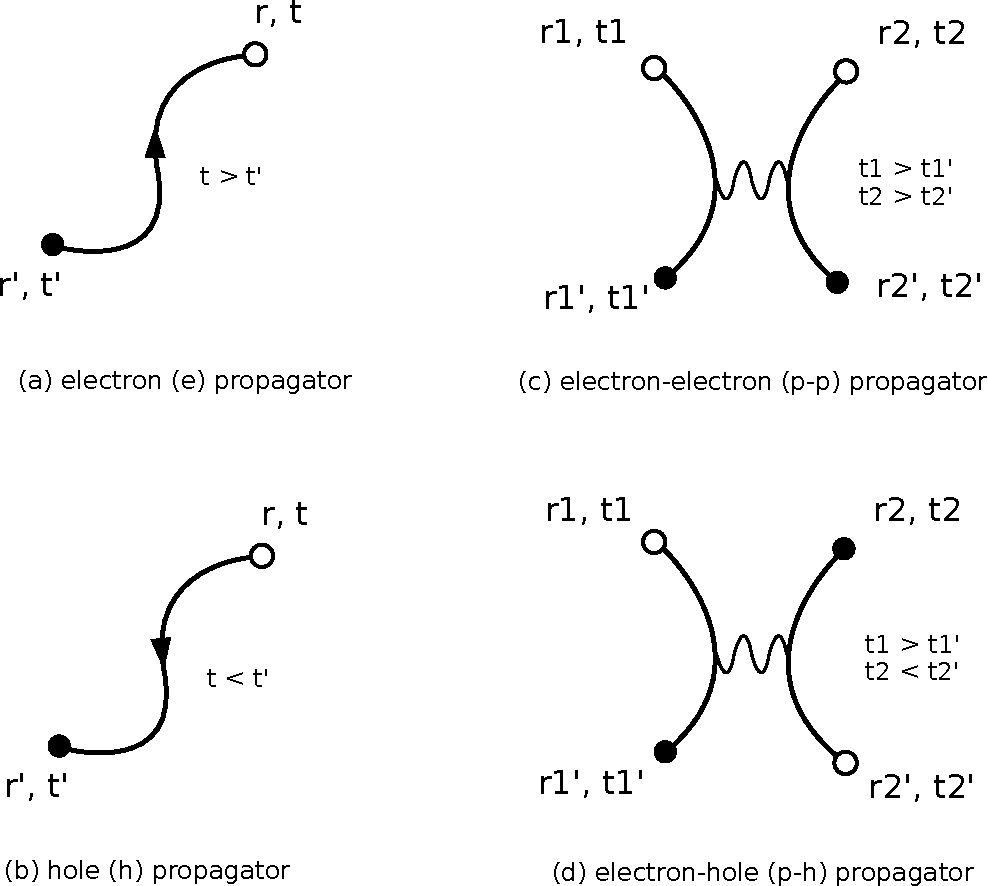
\includegraphics[scale=0.6]{Pics/PROP}
\caption{Hierarchy of Green's functions}
\label{fig:PROP}
\end{figure}

\subsubsection{One-electron Propagator}

To see how GFs can be used for excited state analysis, consider the 1-electron propagator in the time domain
\begin{equation}
G_{pq}(t,t') = - i\Theta(t-t') \sbra{\Psi_0} \hat{T}(a_p[t]a
_q\pdg[t']) \sket{\Psi_0}
\end{equation}
\noindent with $\Theta$ as the Heaviside step function, and the time-ordering operator 
\begin{equation}
\hat{T} = \left\lbrace \begin{matrix}
a_p[t] a_q\pdg[t'] \quad \textrm{for } t > t' \\
-a_q\pdg[t'] a_p[t] \quad \textrm{for } t < t'
\end{matrix}
\right.
\end{equation}
\noindent which plays the role of conserving symmetry with respect to time. It is useful to switch to the energy representation of the GF by Fourier transformation
\begin{equation}
G_{pq} (\omega) = \underbrace{ \sum_n \frac{
	\sbra{\Psi_0} c_p \sket{\Psi_n^{N+1}}			    \sbra{\Psi_n^{N+1}} c_q \pdg \sket{\Psi_0} 
}{
	\omega + E_0 - E_n^{N+1} + i \eta
}
}_{\text{$G^{+}(t,t')$}} + 
\underbrace{
\sum_n \frac{
	\sbra{\Psi_0} c_q \pdg \sket{\Psi_n^{N-1}}			    \sbra{\Psi_n^{N-1}} c_p \sket{\Psi_0}
}{
	\omega + E_n^{N-1} - E_0 - i \eta
}
}_{\text{$G^{-}(t,t')$}}
\end{equation}
\noindent also known as the spectral, energy or Lehmann representation. The superscripts $N+1$ and $N-1$ indicate the addition or removal of an electron form the $N$-electron wave function. The left-hand sum $G^{+}$ describes electron attachment and the right-hand term $G^{-}$ describes electron detachment (ionization). The singularities or \emph{poles} of the spectral representation give the $n$th electron affinity and ionization energy 
\begin{align}
A_n &= E_0 - E_n^{N+1} \\
I_n &= E_n^{N-1} - E_0
\end{align}
\noindent Moreover, the transition strengths (or pole strengths) are given by the spectroscopic factors 
\begin{equation}
x_p^{(n)} = \bra{\Psi_0 } c_p \ket{\Psi_n ^{N+1} }, \quad n \in \left\lbrace N + 1 \right\rbrace
\end{equation}
\begin{equation}
x_p^{(n)} = \bra{\Psi_n^{N-1} } c_p \ket{\Psi_0 }, \quad n \in \left\lbrace N - 1 \right\rbrace
\end{equation}
\noindent By analyzing the 1e-GF, it is therefore possible compute the 1-particle excitation spectrum. 

\subsubsection{Polarization Propagator}

A solution to the single-particle SEQ can be given directly by integrating the GFs. For many-electron systems however, one- and two-particle GFs are only building blocks for many-body propagators. The 1p and 2p GFs allow to introduce the particle-hole response function 
\begin{equation}
R_{pq,uv}(t_1,t_2;t_1',t_2') = G_{pq,uv}(t_1,t_2;t_1',t_2') - G_{pu}(t_1,t_1')G_{qv}(t_2,t_2')
\end{equation}
\noindent also known as the two-particle correlation function. It is the variational derivative of the 1p-GF with respect to an external perturbation $V(t_1,t_2)$, for example in the form of an incoming light quantum \cite{Bay1962}. Similarly to the 1p-GF, analyzing the ph response function gives information on the excited state. It can be evaluated directly via the Bethe-Salpeter equations \cite{Nam1950,Sal1951}, but their dependency on four time variables make them difficult to solve. Fortunately, the same information is already contained in the \emph{polarization propagator} defined by
\begin{equation}
\Pi(t,t') = \lim_{\substack{t_1 \rightarrow t_1'=t \\
t_2 \rightarrow t_2' = t'}} iR(t_1,t_2;t_1',t_2')
\end{equation}  
\noindent The spectral representation of $\Pi$ takes the form
\begin{equation}
\Pi _{p,q;r,s} = \underbrace{ \sum_{n \neq 0} \frac{ 
	\bra{\Psi_0} \hat{c}_q \pdg \hat{c}_p 		\ket{\Psi_n} \bra{\Psi_n} \hat{c}_r \pdg \hat{c}_s \ket{\Psi_0}
}{
	\omega - (E_n - E_0) + i \eta
} }_\text{$\Pi _+(\omega)$} + \underbrace{ \sum_{n \neq 0} \frac{ 
	\bra{\Psi_0} \hat{c}_r \pdg \hat{c}_s \ket{\Psi_n} \bra{\Psi_n} \hat{c}_q \pdg \hat{c}_p \ket{\Psi_0}
}{
	- \omega - (E_n - E_0) + i \eta
} }_\text{$\Pi _-(\omega)$}
\label{eq:POLPROP}
\end{equation}
\noindent Here, the poles correspond to the excitation energies $\omega_n = E_n - E_0$ and the spectroscopic factors give the transition strengths. The polarization propagator is therefore all one needs to evaluate absorption or emission spectra of molecules. The left and right hand terms are related by
\begin{equation}
\Pi(-\omega)_{+}\pdg = \Pi_{-}(\omega)
\end{equation}

Up to this point, the exact wave function was used in the expression for the propagators. To actually be able to compute the propagators, approximations need to be applied. There are a couple of choices. Coupled cluster linear response theory inserts the CC ansatz for the wave function and explicitly evaluates expressions for the polarization propagator truncated to a given level of excitations (LR-CCSD, LR-CCSDT etc.).

Alternatively, the polarization propagator may be approached using perturbation theory.

\subsubsection{Diagrammatic Perturbation}

Similarly to the wave function in RSPT, the polarization propagator can be expanded as
\begin{equation}
\Pi = \Pi^{(0)} + \Pi^({1}) + \Pi^{(2)} + \ldots
\label{eq:PERTPOLPROP}
\end{equation}
\noindent The same partitioning of the Hamiltonian is used as in RSPT
\begin{equation}
\hat{H} = \hat{H}_0 + \hat{U}
\end{equation}
\noindent with the expressions for the wave functions and their energies given in Equations ... and ... 

One may then evaluate the series \ref{eq:PERTPOLPROP} using either Rayleigh-Schrödinger perturbation theory or the Gell-Mann Low theorem \cite{Sch2018} to obtain master equations for $\Pi^{(n)}$. However, these equations are very tedious to solve, even more so than for M{\o}ller Plesset, due to the rapidly increasing number of nested terms for higher $n$. For this reason, diagrams were introduced to better keep track of the contributions at a given level. 

Diagrams were originally conceived by Feynman, and are a pictorial representation of mathematical expressions for particle interactions. Over the years, many different types of diagrams were proposed, such as Goldstone, Abrikosov or Hugenholtz diagrams. Each type has its own set of rules on how to construct them and translate them into formulas for a given problem. There is no formal proof: Feynman first worked out the rules by trial and error \cite{Fey1966}, and later refined the model.

% Bay1962 https://journals.aps.org/pr/abstract/10.1103/PhysRev.127.1391
% Sal1951 E. E. Salpeter and H. A. Bethe, Phys. Rev. 84, 1232 (1951)
% Fey1966 https://science.sciencemag.org/content/153/3737/699

Figure ... shows the Feynman diagrams (in Abrikosov notation) for the polarization propagator up to second order. Each line represents a free particle (electron or hole). Lines with the arrow pointing up are also known as particle lines, while those with the arrow pointing down are known as hole lines. Here, the particle lines represent the time evolution of the electron between $t$ and $t'$. The perturbation $\hat{V}$ is represented by dots in the diagrams, with the total number of dots indicating the perturbation order of the diagram. Each dot contributes a factor of $V_{rs[r's']}=\sbra{rs}\hat{V}\sket{r's'} - \sbra{rs}\hat{V}\sket{s'r'}$ to the mathematical expression of the diagram, where $r,s$ and $r',s'$ are incoming and outgoing fermion lines. Each vertex contributes a free one-particle Green's function $G^0_x(t,t')$. Further rules need to be applied to get the correct sign factors from the direction of the lines. As an example, consider the first order expression of the polarization propagator
\begin{equation}
\Pi^{(1)}_{rs,r's'}(t,t') = \sum_{-\infty}^{\infty} \hat{V}_{rs[r's']}  G^{0}_r(t,t_1) G^0_s(t_1,t) G^0_{r'}(t_1,t') G_{s'}^0(t',t_1) dt_1
\label{eq:SPECTRALORDER1}
\end{equation}
\noindent Equation \ref{eq:SPECTRALORDER1} can then be transformed to the energy representation. Alternatively, Goldstone diagrams can be used where the set of rules directly gives the spectral instead of the time representation. 

\begin{figure}
\centering
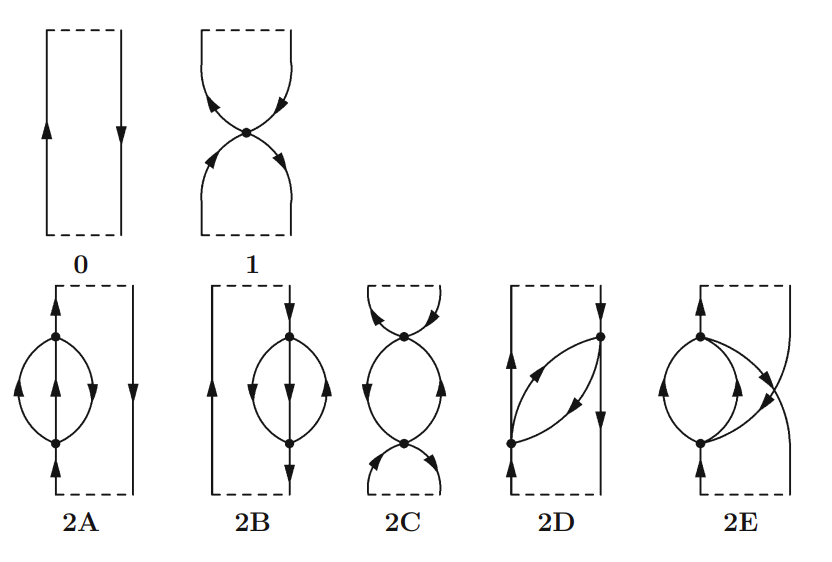
\includegraphics[scale=0.4]{Pics/POLPROP.png}
\label{fig:POLPROP}
\caption{Feynman diagrams in Abrikosov notation for the polarization propagator through second order. Taken from \cite{Sch2018}.}
\end{figure}

\subsection{The ADC scheme}

The polarization propagator cannot be directly "measured". To establish a bridge between theory and experiments, the \emph{transition function} is introduced as
\begin{equation}
T(\omega) = D\pdg \boldsymbol{\Pi}_{+} D 
\end{equation}
\noindent where $\hat{D}$ is an arbitrary operator. The quantity measured during experiments is the \emph{spectral function}, given by
\begin{equation}
f(\omega) = \frac{1}{\pi}Im\{T(\omega)\}
\end{equation}
In the algebraic diagrammatic construction method, the transition function is reformulated as
\begin{equation}
T(\omega) = \mbf{F}\pdg \mbf{\Gamma}(\omega) \mbf{F}
\end{equation}
\noindent where $\mbf{F}$ are the modified transition moments and the non-diagonal matrix $\mbf{\Gamma}$ is given by
\begin{equation}
\mbf{\Gamma}(\omega) = \left[ \omega \mbf{1} - (\mbf{K} + \mbf{C}) \right] = \left[ \omega \mbf{1} - \mbf{M} \right]
\end{equation}
\noindent with the ADC matrix $\mbf{M}$. Writing the transition function, the modified transition moments and $\mbf{M}$ as a perturbation expansion
\begin{align}
T(\omega) &= \sum_{n=0}^{\infty} T^{(n)}(\omega) = \sum_{n=0}^{\infty} D\pdg \boldsymbol{\Pi}_{+}^{(n)} D
\mbf{F} &= \sum_{n=0}^{\infty} \mbf{F}^{(n)} \\
\mbf{M} &= \mbf{K} + \sum_{n=1}^{\infty} \mbf{C}^{(n)}
\end{align} 
\noindent the $n$th order approximations to the transition function read
\begin{align}
T^{(0)}(\omega) &= \mathbf{F}^{(0)\dagger} \left[ \omega \mathbf{1} - \mathbf{K} \right]^{-1} \mathbf{F}^{(0)} \\
\begin{split}
T^{(1)}(\omega) &= \mathbf{F}^{(0)\dagger} \left[ \omega \mathbf{1} - \mathbf{K} \right]^{-1} \mathbf{C}^{(1)} \left[ \omega \mathbf{1} - \mathbf{K} \right]^{-1} \mathbf{F}^{(0)} + \mathbf{F}^{(1)\dagger} \left[ \omega \mathbf{1} - \mathbf{K} \right]^{-1} \mathbf{F}^{(0)} \\
&+ \mathbf{F}^{(0)\dagger} \left[ \omega \mathbf{1} - \mathbf{K} \right]^{-1} \mathbf{F}^{(1)} 
\end{split} 
\\
\begin{split}
T^{(2)}(\omega) &= \mathbf{F}^{(1)\dagger} \left[ \omega \mathbf{1} - \mathbf{K} \right]^{-1} \mathbf{F}^{(1)} + \mathbf{F}^{(0)\dagger} \left[ \omega \mathbf{1} - \mathbf{K} \right]^{-1} \mathbf{C}^{(2)} \left[ \omega \mathbf{1} - \mathbf{K} \right]^{-1} \mathbf{F}^{(0)} \\
&+ \mathbf{F}^{(0)\dagger} \left[ \omega \mathbf{1} - \mathbf{K} \right]^{-1} \mathbf{C}^{(1)} \left[ \omega \mathbf{1} - \mathbf{K} \right]^{-1} \mathbf{C}^{(1)} \left[ \omega \mathbf{1} - \mathbf{K} \right]^{-1} \mathbf{F}^{(0)} \\
&+ \mathbf{F}^{(1)\dagger} \left[ \omega \mathbf{1} - \mathbf{K} \right]^{-1} \mathbf{C}^{(1)} \left[ \omega \mathbf{1} - \mathbf{K} \right]^{-1} \mathbf{F}^{(0)} \\
&+ \mathbf{F}^{(0)\dagger} \left[ \omega \mathbf{1} - \mathbf{K} \right]^{-1} \mathbf{C}^{(1)} \left[ \omega \mathbf{1} - \mathbf{K} \right]^{-1} \mathbf{F}^{(1)}
\end{split}
\end{align}
\noindent By comparing the above $n$th order expression of the transition operator $T(\omega)^{(n)}$ with the mathematical expression of $\mbf{D}\pdg \mbf{\Pi}(\omega) \mbf{D}$ derived using the diagrammatic perturbation of the polarization propagator, algebraic expressions can be \emph{constructed} for the transition moments $\mbf{F}$, and the matrices $\mbf{K}$ and $\mbf{C}$, hence the name algebraic diagrammatic construction.

\subsection{Structure of the ADC matrix}

At its core, ADC reduces to the eigenvalue problem
\begin{equation}
\mbf{M}\mbf{X} = \mbf{X}\boldsymbol{\Omega}
\label{eq:ADCEVAL}
\end{equation}
\noindent The solution gives the vertical excitation energies $\boldsymbol{\Omega}$ and the eigenvectors $\mbf{X}$. Figure \ref{fig:ADCMAT} shows the structure of the ADC matrix $\mbf{M}$ up to third order. Each second level $n$ adds an additional higher excitation manifold to the matrix. ADC(0) and ADC(1) include only singles, while ADC(2) and ADC(3) also include doubles.

The ADC(0) matrix contains only the Hartree-Fock orbital energy differences:
\begin{equation}
M^{(0)}_{ia,jb} = K_{ia,jb} = \delta_{ij}\delta_{ab} (\eps_i - \eps_a) 
\end{equation}
\noindent The ADC(1) matrix adds the first order expression for $\mbf{C}$, and is identical to the CIS matrix:
\begin{equation}
M^{(1)}_{ia,jb} = K_{ia,jb} + C_{ia,jb}^{(1)} = \delta_{ij}\delta_{ab} (\eps_i - \eps_a) - \sbra{ij}\sket{ab}
\end{equation} 
\noindent The ADC(2) matrix has additional second order contributions to the p-h block, and approximates the 2h-1p, 1h-2p to first order and the 2p-2h to zeroth order. 
\begin{align}
C_{ijab}^{(2)} &= C_{ijab}^{(2)A} + C_{ijab}^{(2)B} + C_{ijab}^{(2)C} 
\\
C_{ia,jkcl}^{(1)} &= \sbra{kl} \sket{id} \delta_{ac} - \sbra{kl} \sket{ic} \delta_{ad} - \sbra{al} \sket{cd} \delta_{ik} + \sbra{ak} \sket{cd} \delta_{il} 
\\
C_{iajb,kc}^{(1)} &= \sbra{kb} \sket{ij} \delta_{ac} - \sbra{ka} \sket{ij} \delta_{bc} - \bra{ab} \sket{cj} \delta_{ik} + \sbra{ab} \sket{ci} \delta_{jk} 
\\
K_{iajb,kcld} &= (\epsilon_a - \epsilon_i + \epsilon_b - \epsilon_j) \delta_{ac} \delta_{bd} \delta_{ik} \delta_{jl} 
\end{align}

\noindent with

\begin{align}
C_{ijab}^{(2)A} &= \frac{1}{4} \delta_{ij} \sum_{ckl} \left[  \hat{t}_{ackl} \bra{kl} \sket{bc}  +  \bra{ac} \ket{kl} \hat{t}_{klbc}\right] \\
C_{ijab}^{(2)B} &= \frac{1}{4} \delta_{ab} \sum_{cdk} \left[ \hat{t}_{cdik} \bra{jk} \ket{cd} + \bra{cd} \ket{ik} \hat{t}_{jkcd} \right] \\
C_{ijab}^{(2)C} &= - \frac{1}{2} \sum_{ck} \left[ \hat{t}_{acik}  \bra{jk} \ket{bc} + \bra{ac} \ket{ik} \hat{t}_{jkbc} \right] 
\end{align}

and the anti-symmetrized MP2 amplitudes

\begin{equation}
\hat{t}_{ijab} = \frac{\sbra{ij}\sket{ab}}{\eps_a + \eps_b - \eps_i - \eps_j}
\end{equation}

\begin{figure}
\centering
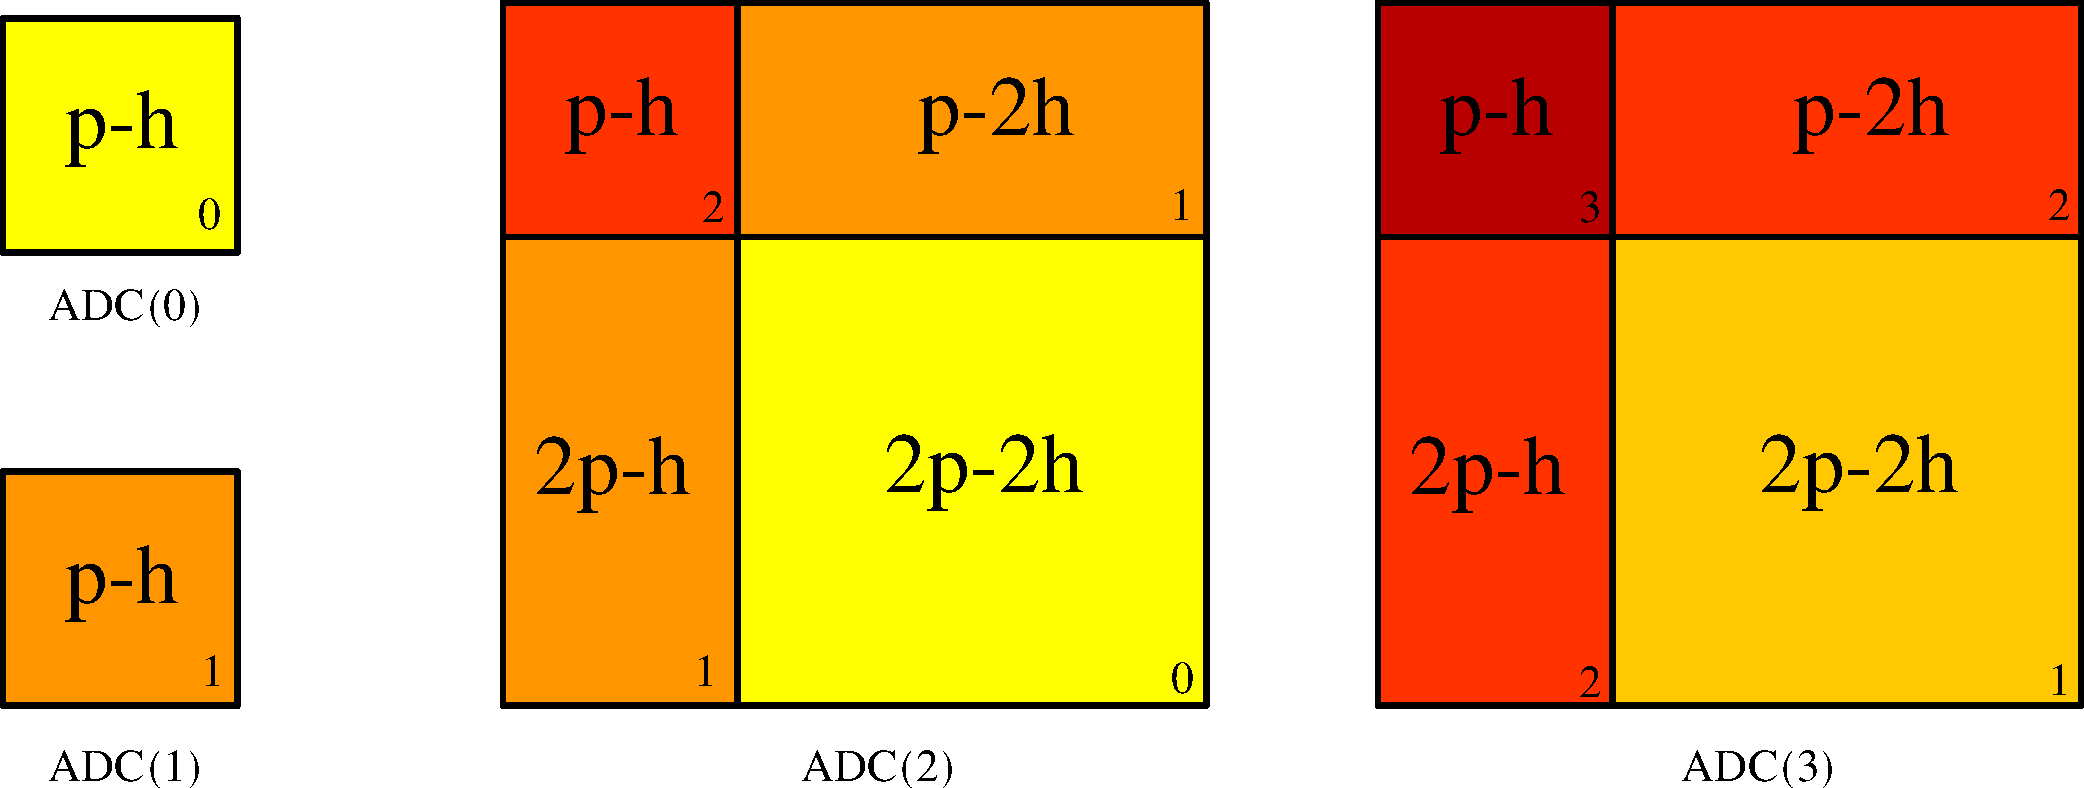
\includegraphics[scale=0.4]{Pics/ADCMAT2}
\caption{Structure of the ADC matrix from zeroth through third order. The number in each block indicates the perturbation order.}
\label{fig:ADCMAT}
\end{figure}

Approximating the 2p-2h block to first order in the ADC(2) matrix, i.e. swapping the 2p-2h block with the one from the ADC(3) matrix, gives the so-called extended ADC(2) scheme (ADC(2)-x). It is an \emph{ad-hoc} extension without rigorous theoretical justification \cite{Tro1995}.  

\subsection{Solving the Eigenvalue Problem \label{sec:ADC_DAV}}

The eigenvalue problem \ref{eq:ADCEVAL} is typically solved using the Davidson procedure to extract the first few eigenvalues, analogous to configuration interaction. Rather than constructing the whole ADC matrix, closed expressions are derived for the matrix-vector products of the different blocks with a general trial vector $\mbf{u}$. For computational considerations, the matrix-vector product is split into its individual components which are then multiplied by the sub-blocks of the ADC matrix. In the case of ADC(2) and ADC(3), the components are limited to singles and doubles contributions:
\begin{align}
r_{ia} &= A_{ia,jb} u_{jb} + A_{ia,jbkc} u_{jbkc} \\
r_{iajb} &= A_{iajb,kc} u_{kc} + A_{iajb,kcld} u_{kcld} 
\end{align}

While the Davidson procedure allows to circumvent storing the whole ADC matrix, the storage of the trial vectors can still be a major memory bottle-neck for ADC(2) and beyond. At second and third order, the doubles part of the vectors scale with $n_{occ}^2n_{vir}^2$, and take up as much space as the MP2 amplitudes. As the Davidson subspace grows, so does the number of trial vectors. Techniques such as \emph{subspace collapse} (Section \ref{sec:DAV}) impose a maximum to the number of trial vectors held in memory, which helps to better estimate the total storage size needed by an ADC calculation, although it increases the total number of iterations to convergence.

An alternative technique to reduce the memory footprint of the Davidson diagonalization is \emph{doubles-folding}. Consider the doubles part of the MVP which is computed as
\begin{align}
r_{iajb} &= A_{iajb,kc} u_{kc} + A_{iajb,kcld} u_{kcld} = \omega u_{iajb}
\end{align}
\noindent By refactoring the above expression, the doubles component of $\mbf{u}$ can be reformulated in terms of its singles component as
\begin{equation}
u_{iajb} = \frac{A_{iajb,kc} u_{kc}}{\omega - A_{iajb,iajb}} 
\label{eq:DS}
\end{equation}
\noindent This technique is limited to ADC(2) only, where the doubles-doubles block is diagonal. Substituting \ref{eq:DS} into the singles expression of the MVP, and using the explicit formulas for the doubles-doubles block gives
\begin{equation}
r_{ia} = A_{ia,jb} u_{jb} + A_{ia,jbkc} \frac{A_{jbkc,ld} u_{ld}}{\omega - \eps_j - \eps_k + \eps_b + \eps_c} 
\end{equation}
\noindent The doubles part of the MVP is computed on-the-fly and does not need to be explicitly stored, reducing the overall memory requirements of the Davidson diagonalization to $n_{occ}n_{vir}$. Doubles-folding corresponds to a multiplication of the singles vectors with an \emph{effective} ADC matrix which depends on the eigenvalue $\omega$
\begin{equation}
\mbf{r}_{\mu_1} = \mbf{A}(\omega)_{\mu_1\nu_1} \mbf{u}_{\nu_1} 
\end{equation}
\noindent One drawback of doubles-folding is that a modified Davidson procedure is necessary to solve this \emph{pseudo} eigenvalue problem (see \ref{seq:DAV}) due to the dependence on the excitation energy $\omega$.

\subsection{Intermediate states}

An alternative route to deriving the ADC working equations is via the intermediate state representation 
\cite{Sch1991,Sch2004,Kni2012}.
%(refs 55, 63, 77, 78 Andreas). 

The previous derivation showed that the eigenvalues of the ADC matrix $\mbf{M}$ correspond to the excitation energies, and that it can be expanded in a perturbation series. These features suggest that $\mbf{M}$ is a representation of the energy-shifted Hamiltonian
\begin{equation}
\mbf{M} = \mbf{H} - E_0
\end{equation}
\noindent with the matrix elements 
\begin{equation}
M_{IJ} = -\sbra{\tPsi_I} \hat{H} - E_0 \sket{\tPsi_J}
\label{eq:ISMATELE}
\end{equation}
\noindent Here, the space of the shifted Hamiltonian is spanned by a set of \emph{intermediate states}. Starting from the set of \emph{correlated excited} (CE) states
\begin{equation}
\sket{\Psi^{\#}_I} = \hat{C}_I \sket{\Psi_0} 
\end{equation}
\noindent with the excitation operators
\begin{equation}
\{\hat{C}_I\} = \{ a_a\pdg a_i; a_b\pdg a_j c_a\pdg c_i; \ldots \}
\end{equation}
\noindent the intermediate states are obtained by a step-wise Gram-Schmidt orthogonalization of the CE states. The ground state $\sket{\Psi_0}$ is approximated by MPPT. Constructing the intermediate states from the MP$n$ ground state wave function and evaluating the matrix elements according to \ref{eq:ISMATELE} gives the $n$th order ADC matrix. For this reason, ADC is also known as "excited state method for M{\o}ller-Plesset". 

\subsection{Spin-Opposite Scaled ADC \label{sec:SOSADC}}

The spin-opposite scaling method previously applied to MP2 and CC2 can be expanded to ADC(2) as well.    There are two version of SOS-ADC(2): the version which will be referred to as "standard" SOS-ADC(2) derived from the SOS-CC2 linear response equations \cite{Win2011}, and ISR-SOS-ADC(2) derived from SOS-MP2 using the intermediate state representation \cite{Kra2013}. Standard SOS-ADC(2) introduces the following modifications to the ADC(2) matrix:
\begin{enumerate}
\item The same-spin contributions of antisymmetrized MP2 amplitudes are ignored, and the opposite-spin components are scaled up:
\begin{equation}
\hat{t}_{IAJB}^{SOS} = c_{os} \hat{t}_{IAJB} \left( 1 - \delta _{\sigma (I) \sigma (J)} \right)
\label{eq:SOSAMPLITUDES}
\end{equation}
where $\sigma (x)$ gives the spin of $x$, and with the amplitudes given by
\begin{equation}
\hat{t}_{IAJB} = \frac{\bra{IJ}{}\ket{AB}}{\epsilon_A + \epsilon_B - \epsilon_I - \epsilon_J}
\end{equation}
\item All same-spin entries of the 2p-1h and 1p-2h blocks of the ADC(2) matrix are deleted ($\alpha\alpha\alpha\alpha$ and $\beta\beta\beta\beta$), and the  remaining blocks are scaled up:
\begin{equation}
M_{ia,kcld} = c_{osc} \left( \bra{kl}{}\ket{id} \gd_{ac} - \bra{kl}{}\ket{ic} \delta_{ac} - \bra{al}{}\ket{cd} \delta_{ik} + \bra{ak}{}\ket{cd} \delta_{il} \right) \left( 1 - \delta_{\sigma (k) \sigma (l)} \right)
\end{equation}
\begin{equation}
M_{iajb,kc} = c_{osc} \left( \bk{kb}{ij} \gd_{ac} - \bk{ka}{ij} \gd_{bc} - \bk{ab}{cj} \gd_{ik} + \bk{ab}{ci} \gd_{jk} \right) \left( 1 - \gd_{\gs (i) \gs (j)} \right)
\end{equation}
\noindent where $c_{osc}$ is the opposite-spin coupling constant, typically set to 1.15 \cite{Kra2013} or 1.17 (diss).
\end{enumerate}

\noindent For open-shell molecules, this drastically reduces the size of the matrix, reducing the prefactor of the method. By applying density fitting, the total scaling can be further reduced by an order of magnitude \cite{Win2011}.

ISR-SOS-ADC(2) does not modify the off-diagonal blocks of the ADC(2) and only replaces the amplitudes as in Equation \ref{eq:SOSAMPLITUDES}, and therefore offers no substantial improvement. 

% 85 https://www.sciencedirect.com/science/article/abs/pii/S030101041100423X
% 86 https://aip.scitation.org/doi/abs/10.1063/1.4776675

\FloatBarrier

\subsection{Performance and Accuracy}

Table \ref{tab:ADCSTATS} lists the formal scaling, mean errors and standard deviation of excitation energies for the ADC($n$) methods. ADC(2), similarly to MP2, offers an economical way of computing excited state properties compared to other excited state methods with similar accuracy. ADC(2)-x and ADC(3) have the same scaling factor, but ADC(2)-x has a lower prefactor.  

The ADC methods offer high accuracy and high precision on the order of a few tenths of eV . The SOS method can significantly reduce the errors, but it should be kept in mind that the spin coefficients were fitted to the benchmark set, and similar accuracy is not guaranteed for other systems.

\begin{table}[h]
\centering
\begin{tabular}{llll}
\hline
Method & Scaling & Singlets & Triplets \\ \hline
ADC(2) & $\ccpx{5}$ & 0.22 $\pm$ 0.38 (62) & 0.12 $\pm$ 0.16 (62) \\
SOS-ADC(2) & $\ccpx{5}$ & 0.00 $\pm$ 0.15 (87) & 0.06 $\pm$ 0.10 (87) \\
ADC(2)-x & $\ccpx{6}$ & -0.70 $\pm$ 0.37 (62) & -0.55 $\pm$ 0.20 (62) \\
SOS-ADC(2)-x & $\ccpx{6}$ & -0.11 $\pm$ 0.18 (87) & -0.04 $\pm$ 0.12 (87) \\
ADC(3) & $\ccpx{6}$ & 0.12 $\pm$ 0.28 (64) & -0.18 $\pm$ 0.16 (64) \\ \hline  
\end{tabular}
\caption{Mean absolute errors (MAE) and deviations (in eV) for closed-shell molecules at various levels of theory. $^a$ \cite{Har2014}, $^b$ \cite{Kra2013}, $^c$ \cite{Tro2006}}
\label{tab:ADCSTATS}
\end{table}

\section{Response Theory}

Response theory is a popular tool similar to propagators that provides methods for computing the response of a molecule to an external, time-dependent perturbation, such as an electromagnetic field. It can be applied to different levels of theory, such as Hartree-Fock, DFT or Coupled Cluster, to gain information on various excited state properties.

\subsection{Exact Response Theory}

Consider a molecular system described by the time-independent Hamiltonian $\hat{H}_0$ with eigenfunctions $\ket{\Psi_0}$ exposed to
an external perturbation $\hat{V}$ given by \cite{Koc1990}
\begin{equation}
\hat{V}(t) = \int_{-\infty}^{\infty} \hat{V}^{\omega} e^{i\omega t  } d\omega
\end{equation}
\noindent where $\hat{V}^{\omega}$ is the representation of the external perturbation in the frequency domain, and $\epsilon$ is a real positive infinitesimal. It has the role of slowly "switching on" the perturbation as time progresses. For $t\rightarrow -\infty$, the perturbation is zero, and at $t \rightarrow \infty$, the perturbation is fully applied. This slow gradual switching makes sure that the process is \emph{adiabatic}.

The time-dependent wave function may be expanded in orders of the perturbation $\hat{V}(t)$ as
\begin{equation}
\sket{\Psi (t)} = \sket{\Psi_0} + \sket{\Psi^{(1)}(t)} + \sket{\Psi^{(2)}(t)} + \ldots
\end{equation}
\noindent which can be determined using Ehrenfest's theorem. Using this wave function expansion, the expectation value of a time-independent operator $\hat{A}$ reads
\begin{equation}
\begin{split}
\sbra{\Psi (t)} \hat{A} \sket{\Psi (t)} = & \sbra{\Psi_0} \hat{A} \sket{\Psi_0} + \int_{-\infty}^{\infty} 
\underbrace{ \langle\langle \hat{A}; \hat{V}^{\omega_1}
\rangle\rangle}_{\text{linear response}} 
e^{(-i\omega_1 + \eps)t} d\omega_1 \\
&+ \frac{1}{2} \int_{-\infty}^{\infty} \int_{-\infty}^{\infty}
\underbrace{ \langle\langle \hat{A}; \hat{V}^{\omega_1},\hat{V}^{\omega_2} \rangle\rangle 
}_{\text{quadratic reponse}}
e^{-i(\omega_1+\omega_2) + 2\eps)t} d\omega_1 d\omega_2  + \ldots
\end{split}
\label{eq:TIMEEXP}
\end{equation}

\noindent The expansion coefficients $\langle\langle \hat{A}; \cdot \rangle\rangle$ are known as \emph{response functions}. Different orders (linear, quadratic...) describe different processes. The linear response function may be used to describe single-photon absorption and polarizability, while the quadratic response function is needed to describe two-photon absorption and hyperpolarizability. 

The spectral representation of the linear response function takes the form
\begin{equation}
\langle\langle \hat{A}; \hat{B}
\rangle\rangle = \sum_k \frac{
	\sbra{\Psi_0}\hat{A}\sket{\Psi_k} \sbra{\Psi_k} \hat{B} \sket{\Psi_0}
}{
	\omega - E_n + E_0
} - \frac{ 
	\sbra{\Psi_0}\hat{B}\sket{\Psi_k} \sbra{\Psi_k} \hat{A} \sket{\Psi_0}
}{
	\omega + E_n - E_0
}
\end{equation}

\noindent and can be analyzed similarly to the polarization propagator: the poles of the function give the excitation energy
\begin{equation}
\omega_i = E_i - E_0
\end{equation}
and the residues give information about the transition moments 
\begin{equation}
\lim_{\omega \rightarrow  \omega_i} (\omega - \omega_i) \langle\langle \hat{A}; \hat{B} \rangle \rangle = \sbra{\Psi_0}\hat{A}\sket{\Psi_i} \sbra{\Psi_i} \hat{B} \sket{\Psi_0}
\end{equation}
for the $i$th excited state. The linear response function and the polarization propagator are related by \cite{Sch2018}
\begin{equation}
\langle\langle \hat{A}; \hat{B}
\rangle\rangle = \sum_{rsr's'} A_{rs} \mbf{\Pi} B_{r's'}
\end{equation}

The expressions for response functions are exact, and need to be evaluated by introducing approximations. Similar to the ADC scheme, finding the poles and residues of the response function ultimately reduces to an eigenvalue problem of the form
\begin{equation}
\mbf{A}\mbf{v} = \mbf{v}\mbf{\Omega}
\end{equation}
\noindent where $\mbf{A}$ can be symmetric (HF,DFT) or non-symmetric (CC).

\subsection{Time-Dependent Hartree-Fock}

There are many different routes for deriving the expressions for the matrix elements of $\mbf{A}$ for linear response time-dependent Hartree-Fock (TDHF) (cf. \ref{Dre2005}), which all lead to the same eigenvalue problem given by 
\begin{equation}
\begin{bmatrix}
\mbf{A} & \mbf{B} \\
\mbf{B}^* & \mbf{A}^* 
\end{bmatrix} 
\begin{bmatrix}
\mbf{X} \\
\mbf{Y} 
\end{bmatrix}
%= 
%\begin{bmatrix}
%\sbra{HF} \left[ \hat{q},\left[ \hat{H}_0, \hat{q}\pdg \right]\right] \sket{HF} & \sbra{HF} \left[ \hat{q},\left[ \hat{H}_0, \hat{q} \right] \right] \sket{HF}\\
%\sbra{HF} \left[ \hat{q}\pdg,\left[ \hat{H}_0, \hat{q}\pdg \right]\right] \sket{HF} & \sbra{HF} \left[ \hat{q}\pdg,\left[ \hat{H}_0, \hat{q} \right]\right] \sket{HF}
%\end{bmatrix}
= 
\omega 
\begin{bmatrix}
1 & 0 \\
0 & -1
\end{bmatrix}
\begin{bmatrix}
\mbf{X} \\
\mbf{Y} 
\end{bmatrix}
\label{eq:TDSCF}
\end{equation}
\noindent where $\mbf{A}$ is the matrix of single excitations, and $\mbf{B}$ couples the excitations with the de-excitations. The matrix elements are given by
\begin{align}
A_{IA,JB} &= \delta_{IA,JB} (\eps_A - \eps_I) + \sket{IJ}{AB} \\
B_{IA,JB} &= \sket{IJ}{AB}
\end{align}
\noindent Setting the coupling block $\mbf{B}$ to zero, the TDHF equations reduce to the CIS equations. Even if TDHF can therefore be seen as an extension to CIS, it does not give a considerable improvement. Over the years, it has fallen into disuse.

Linear response TDHF is equivalent to the \emph{random phase approximation}. 

% 2 McWeeny, R.; Sutcliffe, B. T. Methods of Molecular Quantum Mechanics; Academic Press: London, 1969
% Fetter, A. L.; Walecka, J. D. Quantum Theory of Many-Particle Systems; McGraw-Hill: New York, 1971
% Thouless, D. J. The Quantum Mechanics of Many Body Systems; Academic Press: New York, 1972.
% Dreuw, Andreas; Head-Gordon, Martin (2005). Single-Reference ab Initio Methods for the Calculation of Excited States of Large Molecules. , 105(11), 4009–4037.         doi:10.1021/cr0505627     

\subsection{Time-Dependent DFT}

The foundations of time-dependent DFT  will not be discussed here. The reader is referred to \cite{Dre2005} and references therein for more details. 

The TDDFT linear response equations are similar in structure to TDHF, reducing to the same eigenvalue problem \ref{eq:TDSCF}, with two different blocks $\mbf{A}$ and $\mbf{B}$ given by
\begin{align}
A_{IA,JB} &= \delta_{IA,JB} (\eps_A - \eps_I) + \sbraket{IJ}{AB} +  \sbra{IJ}\hat{f}_{xc} \sket{AB}  \\
B_{IA,JB} &= \sbraket{IJ}{AB} + \sbra{IJ}\hat{f}_{xc} \sket{AB}
\end{align}
\noindent Here, the exchange contributions are replaced by the so-called \emph{xc kernel}. In the adiabatic local density approximation (ALDA), the time dependent xc kernel is substituted by a time-independent kernel 
\begin{equation}
\sbra{IJ}\hat{f}_{xc} \sket{AB} = \int \phi^*_i(\mbf{r}) \phi_j(\mbf{r}') \frac{\partial^2 E_{xc}}{\partial\rho(\mbf{r})\rho(\mbf{r}')} \phi_a (\mbf{r}) \phi_b^*(\mbf{r}')
\end{equation}
\noindent which allows the use of standard xc functionals for the ground state. 

Since its introduction, TDDFT has evolved to become the most prominent method for computing excited state energies and transition moments. It has a computational cost on the same order as CIS, with an error of $\approx$ 0.3 eV \cite{Lau2013} for low-lying valence states. However TDDFT is not a panacea: excitation energies for Rydberg states, valence states of molecules with extended $\pi$-systems, doubly excited states and charge-transfer states exhibit errors on the order of several eV.

% Dreuw, Andreas; Head-Gordon, Martin (2005). Single-Reference ab Initio Methods for the Calculation of Excited States of Large Molecules. , 105(11), 4009–4037.         doi:10.1021/cr0505627     

% A. D. Laurent and D. Jacquemin, Int. J. Quantum Chem. , 2019 (2013)

\subsection{Coupled Cluster}

The derivation of the coupled cluster response equations is again a very lengthy and complex process \cite{Koc1990,Chr1998}. The most important steps will be summarized in this section.

For a molecular system in the presence of a static external perturbation, such as a constant electric or magnetic field with strength parameter $\lambda$, the Hellmann-Feynman theorem relates the expectation value of $\hat{X}_{\lambda}$ to the energy derivative by
\begin{equation}
\frac{\partial E}{\partial \lambda_x} = \sbra{\Psi}\frac{\partial \hat{H}}{\partial \lambda_x} \sket{\Psi} = \sbra{\Psi}\hat{X} \sket{\Psi}
\label{eq:HELLFEYN}
\end{equation}
\noindent By perturbation expansion of $\hat{X}$, the $n$th order property can then be related to the $n$th order derivative of the wave function energy, which is in most cases is more readily derived than the expectation value. For time-dependent perturbations, the theorem can be reformulated as 
\begin{equation}
\frac{\partial \{Q\}_T}{\partial \lambda_x} = \sbra{\Psi(t)} \hat{X}(t) \sket{\Psi(t)} 
\end{equation}
\noindent where $\{Q\}_T$ is the time-averaged \emph{quasi-energy} given by
\begin{equation}
\{Q\}_T = \frac{1}{T} \int_0^T \sbra{\Psi(t)} (\hat{H} - i\frac{\partial}{\partial t})\sket{\Psi(t)}
\label{eq:HELLFEYN2}
\end{equation}
\noindent The time-averaged quasi-energy is the analog of the ground state energy for static perturbations in Equation \ref{eq:HELLFEYN}. Using the perturbation expansion \ref{eq:TIMEEXP} for the operator, the first, second, ... derivative of the quasi-energy can be related to the linear, quadratic ... response function. Similarly to the energy derivative, expressions for quasi-energy derivatives are more easily evaluated. The CC response equations are then obtained by constructing a Lagrangian of the CC quasi-energy. 

Analysis of the CC response equations leads to the non-symmetric eigenvalue problem
\begin{align}
\mbf{A}\mbf{R} &= \mbf{\Omega}\mbf{R} \\
\mbf{L}\mbf{A} &= \mbf{R}\mbf{\Omega} 
\end{align} 
\noindent where $\mbf{R}$ and $\mbf{L}$ are the right and left eigenvectors respectively.

Analogous to ground state calculations, a hierarchy of CC response methods is obtained by truncating the excitation operator $\hat{T}$ to singles, doubles, triples, ... to yield CCS-LR, CCSD-LR, CCSDT-LR. Approximate CC methods may also be used, such as CC2, CC3 or CCSD(T). The formal scaling of the different methods is equal to their respective scaling for ground states, although with a higher prefactor. CC2 excitation energies are similar in accuracy to ADC(2). CCSD is better than ADC(2), and CC3 is slightly better than ADC(3) \cite{Loo2020}. 

% https://pubs.acs.org/doi/pdf/10.1021/acs.jpclett.9b03652

\subsection{Connection between ADC(2) and CC2-LR} 

An interesting relationship can be established between ADC(2) and CC2-LR \cite{Hf2005}. Consider the expression for the CC2 Jacobian:
\begin{equation}
\mbf{A}^{CC2-LR} = \left( \begin{matrix}
\sbra{\mu_1} \left[ (\hat{\bar{H}} + \left[ \smash{ \hat{\bar{H}},\hat{T}_2} \right]), \tau_{\nu_1} \right] \sket{HF} &  \sbra{\mu_1} \left[ \hat{\bar{H}}, \tau_{\nu_2} \right] \sket{HF} \\
\sbra{\mu_2} \left[ \hat{\bar{H}}, \tau_{\nu_1} \right] \sket{HF} & \sbra{\mu_2} \left[ (\hat{\bar{H}} + \left[ \smash{ \hat{F},\hat{T}_2} \right]), \tau_{\nu_2} \right] \sket{HF}
\end{matrix}
\right)
\end{equation}

\noindent where $\mu_1$, $\mu_2$ are the single and double excitation manifolds. By replacing the similarity-transformed Hamiltonian $\hat{\bar{H}}$ by the Hamiltonian itself, the CIS(D) matrix reads
\begin{equation}
\mbf{A}^{CIS(D)} = \left( \begin{matrix}
\sbra{\mu_1} \left[ (\hat{\bar{H}} + \left[ \smash{ \hat{H},\hat{T}_2} \right]), \tau_{\nu_1} \right] \sket{HF} &  \sbra{\mu_1} \left[ \hat{H}, \tau_{\nu_2} \right] \sket{HF} \\
\sbra{\mu_2} \left[ \hat{H}, \tau_{\nu_1} \right] \sket{HF} & \sbra{\mu_2} \left[ (\hat{H} + \left[ \smash{ \hat{F},\hat{T}_2} \right]), \tau_{\nu_2} \right] \sket{HF}
\end{matrix}
\right)
\end{equation}

\noindent CIS(D) is a second-order perturbative correction of CIS which includes doubles contributions \cite{Hea1994} scaling with $\ccpx{5}$. The ADC(2) matrix is then obtained by symmetrization
\begin{equation}
\mbf{A}^{ADC(2)} = \frac{1}{2} \left(\mbf{A}^{CIS(D)} + (\mbf{A}^{CIS(D)})\pdg \right)
\end{equation}
\noindent This relationship is especially useful for easily deriving approximate methods for ADC(2) from CC2, such as SOS-ADC(2), or local ADC(2).

% Koc1990 https://aip.scitation.org/doi/pdf/10.1063/1.458814
% Chr1997 https://onlinelibrary.wiley.com/doi/epdf/10.1002/%28SICI%291097-461X%281998%2968%3A1%3C1%3A%3AAID-QUA1%3E3.0.CO%3B2-Z
% Hat2005 https://www.sciencedirect.com/science/article/abs/pii/S0065327605500030?via%3Dihub
% Hea1994 https://www.sciencedirect.com/science/article/abs/pii/0009261494000700?via%3Dihub

\section{Equation-of-Motion Coupled Cluster}

An alternative way for describing the molecular response to an external field using coupled cluster is via the equation-of-motion (EOM) ansatz \cite{Gee1989,EMr1981,Sta1993,Sta1994,Kry2008}. In the EOM approach, the target excited (R) and de-excited (L) wave functions are parameterized as 
\begin{align}
\sket{\Psi_R} &= e^{\hat{T}} \hat{R} \sket{\Psi_0} \\
\sbra{\Psi_L} &= \sbra{\Phi_0} \hat{L} e^{-\hat{T}} 
\end{align}
\noindent with the excitation and de-excitation operators $\hat{R}$ and $\hat{L}$ 
\begin{align}
\hat{R} &= \sum r_{\mu} \hat{\tau}_{\mu} \\
\hat{L} &= \sum l_{\mu} \hat{\tau}_{\mu}
\end{align}
\noindent where $r$ and $l$ are the excitation and de-excitation cluster amplitudes. The exact form of $\hat{R}$ and $\hat{L}$ depend on the nature of the reference and final states. The most common uses of EOM are for the calculation of excitation energies and ionization potentials. In the case of EOM-EE, with $\Psi_0$ taken as the Hartree-Fock wave function, $\hat{R}$ and $\hat{L}$ conserve the number of electrons and are given as
\begin{align}
\hat{R}_{EE} &= r_0 + \sum_{IA} r_I^A a_A\pdg a_I + \frac{1}{4} \sum_{IAJB} r_{IJ}^{AB} a_A\pdg a_I a_B\pdg a_J + \ldots \\
\hat{L}_{EE} &= l_0 + \sum_{IA} l_I^A a_I\pdg a_A + \frac{1}{4} \sum_{IAJB} l_{IJ}^{AB} a_I\pdg a_A a_J\pdg a_B + \ldots
\end{align}
The (de-)excitation operators can be truncated similar to $\hat{T}$ to yield different approximations (EOM-CCS, EOM-CCSD...). The cluster amplitudes and the excitation energies are obtained 
by solving the non-Hermitian eigenvalue problem 
\begin{align}
\sbra{\mu} \hat{\bar{H}} \hat{R} \sket{HF} &= 0 \\
\sbra{HF \hat{L}} \hat{\bar{H}} - E \sket{HF} &= 0
\end{align}
The excitation energies obtained by solving the LR-CC and EOM-CC eigenvalue problems are identical for pure CC models (CCSD, CCSDT...), but they give different results for transition moments and excited-state properties.

The EOM-CC methods, alongside ADC and CC-LR, are among the most accurate methods available for excited states. 




